\documentclass{ximera}
\input{../preamble}
\addPrintStyle{..}
\begin{document}
	\author{Zomercursus KU Leuven}
	\xmtitle{Complexe getallen}{}
	
	\label{xim:complexe_getallen}
    
Veeltermvergelijkingen hebben niet altijd reële oplossingen. Zo hebben vierkantsvergelijkingen met een negatieve discriminant geen reële wortels. Een erg eenvoudig voorbeeld is de vergelijking $x^2+1=0$ of, anders geschreven, $x^2=-1$. Deze vergelijking heeft geen reële wortels, omdat het kwadraat van een reëel getal nooit negatief kan zijn, en dus nooit gelijk aan $-1$. 

De zogenaamde \textit{complexe getallen} vormen een uitbreiding van de reële getallen. Aan de reële getallen wordt een nieuw 'getal' toegevoegd dat traditioneel $i$ genoemd wordt, en $i$ is \textit{per definitie} een oplossing van de vergelijking $x^2+1=0$. Er geldt dus per definitie dat $i^2=-1$. Het is een hoogst merkwaardig feit dat door een oplossing van deze vergelijking $x^2+1=0$ toe te voegen, ineens \textit{alle} veeltermvergelijkingen met reële coëfficiënten oplossingen blijken te hebben.

\begin{xmuitweiding}[Nieuwe getallen uitvinden, mag dat zomaar?] \nl
Vertrekkend van de natuurlijke getallen, over negatieve getallen en breuken tot bij reële getallen worden in de wiskunde steeds nieuwe soorten getallen toegevoegd (men zou ook kunnen zeggen 'gedefinieerd' of 'uitgevonden'). Het is een merkwaardig fenomeen dat de dingen daarbij steeds eenvoudiger worden. Wiskunde wordt eenvoudiger omdat steeds meer operaties gewoon kunnen worden uitgevoerd: bij de natuurlijke getallen moeten we opletten wanneer het verschil van twee getallen kan genomen worden (want $2-3 \not\in\N$), bij de gehele getallen kunnen we niet altijd delen (want $1/2\not\in\Z$), en bij de rationale getallen kunnen we niet altijd een vierkantswortel nemen (want $\sqrt{2}\not\in\Q$). In zeker opzicht is de vierkantswortel van negatieve getallen de laatste horde die we moeten nemen. Die bestaat niet in $\R$, maar hij bestaat wel in de zogenaamde \textit{complexe getallen} $\C$. Daarbij staat complex gelukkig niet voor \textit{ingewikkeld}, maar voor \textit{samengesteld}. Zoals steeds vergt het wat tijd en een zekere inspanning om vertrouwd te worden met een nieuw begrip.

De complexe getallen ontstaan door een nieuw 'getal' $i$ te definiëren waarvoor \textit{per definitie} geldt dat $i^2=-1$. We zullen zien dat we met dat nieuwe getal gewoon kunnen rekenen zoals we al gewoon zijn met de reële getallen. Verder zal ook blijken dat er een mooie meetkundige interpretatie is van het getal $i$.

%\hyperref[uitw:veld]{Verder} wordt uitgelegd wat wiskundigen \textit{precies} bedoelen met 'iets gedraagt zich als een getal'. Een mogelijk antwoord zal zijn: iets is redelijkerwijs een getal als het beschouwd wordt als een element van een \textit{veld}.  

Complexe getallen spreken zowel tot de verbeelding van de wiskundige als van de ingenieur en de fysicus.  Wiskundigen leggen vooral de nadruk op de eigenschappen van de complexe getallenverzameling en op de hoofdstelling van de algebra. Ingenieurs en fysici  gebruiken ze in verschillende toepassingen zoals systeemtheorie, elektrische netwerken, trillingen en golfverschijnselen.
\end{xmuitweiding}


\begin{definition}\nl
	
%De verzameling van de \textbf{complexe getallen} is per definitie
%$$
%\C =\left\{a+bi\;|\:a,b \in \R\; \Ten \important{i^2=-1} \right\}
%$$ 
Een \textbf{complex getal} is een uitdrukking $a+bi$, met $a,b \in \R$ en waarbij $i^2=-1$. Het symbool $i$ is de \textbf{imaginaire eenheid}. De verzameling van alle complexe getallen noemen we $\C$.

Per definitie zijn twee complexe getallen $a+bi$ en $c+di$ enkel aan elkaar gelijk als $a=c$ en $b=d$.

Een willekeurig complex getal wordt dikwijls genoteerd met $z$. Als $z=a+bi$, dan
\begin{itemize}
\item is $a$ het \textbf{reëel deel} van $z$, genoteerd als $\text{Re}(z) \perdef a$.
\item is $b$ het \textbf{imaginair deel} van $z$, genoteerd als $\text{Im}(z)\perdef b$.
\item Als $b=0$, dan is $z=a$ een \textbf{(zuiver) re\"eel getal} (en $\R$ is dus een deelverzameling van $\C$).
\item Als $a=0$, dan is $z=bi$ een \textbf{(zuiver) imaginair getal}. 
%We noteren de verzameling van die getallen soms als $i\R$.
\end{itemize}
\end{definition}

\begin{example} Volgende uitdrukkingen zijn allemaal complexe getallen:
\begin{xmmulticols}[3]
\begin{enumerate}
\item $2+3i$ 				    % a
\item $42$   				    % b
\item $42i$  				    % c
\item $1+\pi$				    % d
\item $1+i\sqrt{2}$ 		    % e
\item $\dfrac{1-i\sqrt{5}}{2}$  % f
\end{enumerate}
\end{xmmulticols}
De getallen $42$ en $1+\pi$ zijn zuiver reële getallen, en $42i$ is een zuiver imaginair getal. 
\end{example}

\xmsection{Het complexe vlak}\nl

We kunnen met elk complex getal $z=a+bi$ een uniek koppel $(a,b)$ associëren. Op die manier kan een complex getal $z$ ook voorgesteld worden als een punt in het vlak, met $x$-coördinaat $a$ en $y$-coördinaat $b$:

\begin{image}[0.8\textwidth]
	\begin{tikzpicture}[scale=3]%,cap=round,transform canvas={scale=0.5}]
	
	\tikzmath{\hoek = 35; \myc = cos(\hoek); \mys = sin(\hoek); 
		\hoekb = 20;}
	
		% Goniometrische cirkel
%	\draw (0,0) circle (1cm);
	\draw[->] (-0.2,0) -- (1.2,0) node[above] {Re$(z)$};
	\draw[->] (0,-0.2) -- (0,1)   node[right] {Im$(z)$};

	\draw[color=blue,thick] (0:0)  -- (\hoek:1); 
	%
	\draw[color=black] (\hoek:1) node[name=P,circle, fill=black, radius=1pt,scale=0.8] {} node [yshift=2pt,above] {$z=a+bi$} ;  
	%
	\draw[dashed] ({cos(\hoek)},0) node[circle, fill=black, radius=1pt,scale=0.5] {} node[below] {$a$} -- (P);
	\draw[dashed] (0,{sin(\hoek)}) node[circle, fill=black, radius=1pt,scale=0.5] {} node[left] {$b$} -- (P);
	%
	\draw [thick, red,decorate,decoration={brace,amplitude=10pt,mirror},yshift=-5pt](0,0) -- ({cos(\hoek)},0) node[black,midway,yshift=-0.6cm] {\footnotesize $a$};
	%
	\draw [thick, red,decorate,decoration={brace,amplitude=10pt},xshift=-10pt](0,0) -- (0,{sin(\hoek)}) node[black,midway,left,xshift=-8pt] {\footnotesize $b$};
    
    \begin{scope}[xshift=2cm]
    		% Goniometrische cirkel
    %	\draw (0,0) circle (1cm);
    	\draw[->] (-0.2,0) -- (1.2,0) node[above] {$x$};
    	\draw[->] (0,-0.2) -- (0,1)   node[right] {$y$};
    
%    	\draw[color=blue,thick] (0:0)  -- (\hoek:1); 
    	%
    	\draw[color=black] (\hoek:1) node[name=P,circle, fill=black, radius=1pt,scale=0.8] {} node [yshift=2pt,above] {$(a,b)$} ;  
    	%
    	\draw[dashed] ({cos(\hoek)},0) node[circle, fill=black, radius=1pt,scale=0.5] {} node[below] {$a$} -- (P);
    	\draw[dashed] (0,{sin(\hoek)}) node[circle, fill=black, radius=1pt,scale=0.5] {} node[left] {$b$} -- (P);
    	%
    	\draw [thick, red,decorate,decoration={brace,amplitude=10pt,mirror},yshift=-5pt](0,0) -- ({cos(\hoek)},0) node[black,midway,yshift=-0.6cm] {\footnotesize $a$};
    	%
    	\draw [thick, red,decorate,decoration={brace,amplitude=10pt},xshift=-10pt](0,0) -- (0,{sin(\hoek)}) node[black,midway,left,xshift=-8pt] {\footnotesize $b$};
    \end{scope}
	
	\end{tikzpicture}
	\end{image}

Als we het vlak op deze manier bekijken als de verzameling van de complexe getallen, spreken we van het \textbf{complexe vlak}. Het getal $i$ komt daarbij overeen met het koppel $(0,1)$ op de $y$-as.

\begin{basicSkip}
\youtube{Ho_oadFkm1o}  % Bron: SPOC Complexe getallen
\end{basicSkip}

\begin{exercise}
    Schets in het complexe vlak de gebieden omschreven door volgende vergelijkingen:
    \begin{question} 
        $\text{Im}(z) \leq 0$
        \begin{oplossing} Als $z=a+bi$, dan betekent Im$(z) \leq 0$ dat $b \leq 0$ en dat geeft het  halfvlak onder de $x$-as:
            
            \begin{image}[0.5\textwidth]
                \begin{tikzpicture}[scale=0.8, baseline=(current bounding box.north)]
                \draw[dashed] (-5, -3) grid (5, 1);
                \draw[blue, ->, thick] (-5, 0.05) -- (5, 0.05) node[right, black] {Re$(z)$};
                \draw[->, thick] (0, -3) -- (0, 1) node[above] {Im$(z)$};
                
                \draw[white, pattern=north west lines, pattern color=blue] (-5,0) rectangle (5,-3);
                \end{tikzpicture}
            \end{image}
        \end{oplossing}
    \end{question}
    
    \begin{question} 
        $0 \leq \text{Re}(z) \leq 4$
        \begin{oplossing} Deze ongelijkheden bepalen een \textit{verticale} strook, aangezien het reële deel van het complex getal in een interval moet liggen. De randen van de strook behoren tot het geschetste domein.
            
            \begin{image}[0.3\textwidth]
                \begin{tikzpicture}[scale=0.8, baseline=(current bounding box.north)]
                \draw[dashed] (-1, -4) grid (5, 4);
                
                \draw[->, thick] (-1, 0) -- (5, 0) node[right] {Re$(z)$};
                \draw[->, thick] (0, -4) -- (0, 4)   node[above] {Im$(z)$};
                
                \draw[white, pattern=north west lines, pattern color=blue] (0,4) rectangle (4, -4);
                
                % randen toevoegen voor duidelijkheid 
                \draw[blue, thick] (0, -4) -- (0, 4);
                \draw[blue, thick] (4, -4) -- (4, 4);
                \end{tikzpicture}
            \end{image}
        \end{oplossing}            
    \end{question}        
    \end{exercise}

\xmsection{Rekenen met complexe getallen}\nl

Voor complexe getallen kan, met de gebruikelijke rekenregels, de optelling en vermenigvuldiging gedefinieerd worden, waarbij steeds $i^2$ vervangen wordt door $-1$. 
% todo: ref toevoegen naar uitleg in deel over complexe vlak ...?

\begin{definition}[Som en product]\nl
	
Als $a_1,b_1,a_2,b_2\in\R$, en dus $z_1=a_1+b_1 i, z_2=a_2+b_2i \in \C$ geldt:
\begin{align*}
z_1+z_2 = (a_1+b_1i)+(a_2+b_2i) & \perdef (a_1+a_2)+(b_1+b_2)i \\
z_1 \cdot z_2 = (a_1+b_1i)\: \cdot \: (a_2+b_2i) & \perdef a_1 a_2+a_1 b_2i+ a_2 b_1i+b_1b_2\underbrace{i^2}_{ i^2=-1} = (a_1 a_2-b_1 b_2)+(a_1 b_2+a_2 b_1)i
\end{align*}

\end{definition}

Meetkundig is de optelling van complexe getallen hetzelfde als de optelling van vectoren in het vlak: het komt neer op de parallellogramregel:

\begin{image}[0.5\textwidth]
	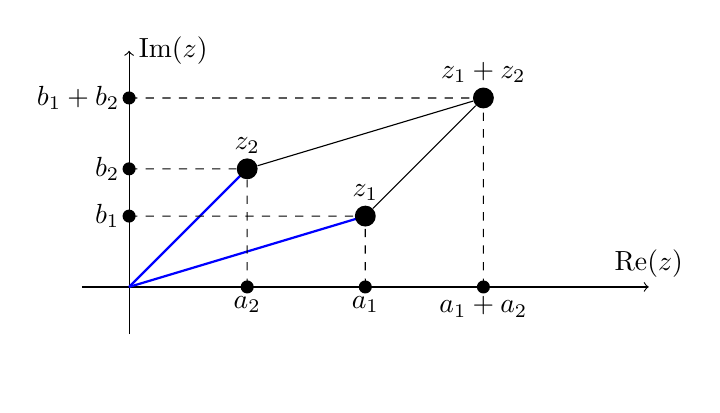
\begin{tikzpicture}[scale=3]%,cap=round,transform canvas={scale=0.5}]
	
	\draw[->] (-0.2,0) -- (2.2,0) node[above] {Re$(z)$};
	\draw[->] (0,-0.2) -- (0,1)   node[right] {Im$(z)$};
	
	\draw[color=blue,thick] (0:0)  -- (1,0.3); 
	\draw[color=blue,thick] (0:0)  -- (0.5,0.5); 
	
	%
	\draw[color=black] (1,0.3) node[name=Z1,circle, fill=black, radius=1pt,scale=0.8] {} node [yshift=2pt,above] {$z_1$} ;  
	\draw[color=black] (0.5,0.5) node[name=Z2,circle, fill=black, radius=1pt,scale=0.8] {} node [yshift=2pt,above] {$z_2$} ;  
	%
	\draw[color=black] (1.5,0.8) node[name=Zs,circle, fill=black, radius=1pt,scale=0.8] {} node [yshift=2pt,above] {$z_1+z_2$} ;  
	%
	\draw[dashed] (1,0)    node[circle, fill=black, radius=1pt,scale=0.5] {} node[below] {$a_1$} -- (Z1);
	\draw[dashed] (0,0.3) node[circle, fill=black, radius=1pt,scale=0.5] {} node[left] {$b_1$} -- (Z1);
	%
	\draw[dashed] (0.5,0) node[circle, fill=black, radius=1pt,scale=0.5] {} node[below] {$a_2$} -- (Z2);
	\draw[dashed] (0,0.5)   node[circle, fill=black, radius=1pt,scale=0.5] {} node[left] {$b_2$} -- (Z2);
	%	
	\draw[dashed] (1.5,0)    node[circle, fill=black, radius=1pt,scale=0.5] {} node[below] {$a_1+a_2$} -- (Zs);
	\draw[dashed] (0,0.8) node[circle, fill=black, radius=1pt,scale=0.5] {} node[left] {$b_1+b_2$} -- (Zs);
	%
	\draw[black] (Z1) -- (Zs);
	\draw[black] (Z2) -- (Zs);
	%
	% onzicktbaar: enkel voor alignment met vorige picture !
	\path [thick, red,decorate,decoration={brace,amplitude=10pt,mirror},yshift=-5pt](0,0) -- (1,0) node[black,midway,yshift=-0.6cm] {};
	
	\end{tikzpicture}
	
	
\end{image}

\begin{remark} \nl
\begin{itemize}
	\item Een complex getal kan per definitie op een unieke manier geschreven worden als $a+bi$, met $a,b\in\R$. Dus $1, i, 1+i, 1+3i$ zijn allemaal complexe getallen die we niet eenvoudiger kunnen schrijven. Maar $2i+3+i, i(1+i)$ en $(1+i)(1-i)$ zijn complexe getallen die we wel eenvoudiger kunnen schrijven als $2i+3+i=3+3i, \quad i(1+i)=i+i^2 =-1+i,\quad  (1+i)(1-i) = 1 - i^2 = 1+1 =2$.
    
    \item Als je twee complexe getallen kan optellen, is het ook eenvoudig om ze van elkaar af te trekken: $(a_1+b_1i)-(a_2+b_2i) = (a_1-a_2)+(b_1-b_2)i$. Je kan twee complexe getallen ook \textit{delen} door elkaar, dit wordt later uitgelegd.
%    maar dat is wat complexer \xmopje{(pun intended)}. Je kan er zelf eens over nadenken, maar we geven hier geen formule voor de deling van complexe getallen. Delen zal verder een eenvoudige toepassing blijken te zijn van de \textit{inverse} van een complex getal.
    
	\item Ingenieurs gebruiken meestal de letter $j$ in plaats van $i$, onder meer om verwarring te voorkomen met de elektrische stroom $i$. Dan geldt dus $j^2=-1$, en $z=a+bj\in\C$.
	
	\item 
	Men kan aantonen dat de verzameling $\C$ \textbf{niet totaal kan geordend worden} zoals $\Q$ of $\R$. Hiermee wordt bedoeld dat het niet mogelijk is om een definitie te vinden voor $a+bi <c+di$ die zou voldoen aan dezelfde eigenschappen als de ongelijkheid $<$ in $\R$ of $\Q$. Je kan van twee complexe getallen dus niet zeggen welk "het kleinste" is.
%	 (Het begrip \textit{modulus} zal verder toch een soort 'grootte' introduceren, maar complexe getallen kunnen 'dezelfde grootte' hebben zonder aan elkaar 'gelijk' te zijn. Die 'grootte' gedraagt zich dus toch erg anders dan de 'orde' op $\R$.)   )
	\\ 
	In het bijzonder heeft het geen betekenis om te vragen of $2+3i$ \textit{positief} of \textit{negatief} is. 
	Zo kan je ook niet zeggen dat $1+i$ \textit{positief} is en $-1-i$ \textit{ negatief}, maar wel dat ze elkaars \textit{tegengestelde} zijn. Hetzelfde geldt zelfs voor $i$: het heeft geen betekenis om te beweren dat $i$ positief is, en $-i$ negatief. Het heeft wel betekenis om te zeggen dat $i$ en $-i$ elkaars tegengestelde zijn.
    
%    \item Voor het reëel en imaginair deel van $z=a+bi$ worden soms andere notaties gebruikt: \\ $a=\Re(z)=\text{Re}(z)=\text{Re}(a+bi)$, en  $b= \Im(z)=\text{Im}(z)=\text{Im}(a+bi)$.
\end{itemize}
\end{remark}

\begin{xmuitweiding}[Meetkundige betekenis van complexe getallen]\nl

Volgende video legt in detail uit hoe complexe getallen \textit{meetkundig} kunnen worden voorgesteld.
In het bijzonder wordt er een interessante meetkundige interpretatie gegeven voor de vermenigvuldiging met $i$.

% Uit de SPOC Complexe Getallen
\youtube{i1aPI3_nia4}

\end{xmuitweiding}


\begin{exercise} \nl 
%	\begin{xmmulticols}
	\begin{question}$(1+2i) + (3+4i)     = \answer[onlineshowanswerbutton]{4+6i}$ \end{question}
	\begin{question}$(1+2i) \cdot (3+4i) = \answer[onlineshowanswerbutton]{-5+10i}$ 
	\begin{oplossing}
	 $(1+2i) \cdot (3+4i) = 3 + 4i + 2i\cdot 3 + 2i \cdot 4i = -5 + 10i$
	\end{oplossing}	
	\end{question}
	\begin{question}$(1+2i) \cdot (1-2i) = \answer[onlineshowanswerbutton]{5}$ 
	\begin{oplossing}
	Haakjes uitwerken, of eenvoudiger via $(a-b)(a+b) = a^2 - b^2$ wat ook geldt voor complexe getallen:
	$$
	(1+2i) \cdot (1-2i) = 1^2 - (2i)^2 = 1 + 4 = 5
	$$
	\end{oplossing}	
	\end{question}
	\begin{question}$(1+2i) \cdot \frac{1-2i}{2} = \answer[onlineshowanswerbutton]{\frac52}$ \end{question}
    \begin{question}$(1+2i) \cdot i = \answer[onlineshowanswerbutton]{-2+i}$ \end{question}
    \begin{question}$i^3 = \answer[onlineshowanswerbutton]{-i}$
	\begin{oplossing}
	$i^3 = i\cdot i^2 = -i$
	\end{oplossing}    
    \end{question}
    \begin{question}$i^4 = \answer[onlineshowanswerbutton]{1}$
	\begin{oplossing}
	$i^4 = i^2\cdot i^2 = (-1) \cdot (-1) = 1$ of $i^4 = (i^2)^2 = (-1)^2 = 1$
	\end{oplossing}    
    \end{question}
%	\end{xmmulticols}
\end{exercise}

\xmsection{Modulus en complex toegevoegde}\nl

Complexe getallen zijn niet alleen 'samengesteld', maar toch ook net iets 'complexer' dan reële getallen. Om ze te bestuderen beschikken we over twee nieuwe begrippen. Het eerste, de \textit{modulus}, is een veralgemening van de absolute waarde van reële getallen. Het tweede, de zogenaamde \textit{complex toegevoegde}, heeft niet direct een analoog voor de reële getallen:

\begin{definition}[Modulus en complex toegevoegde] \nl 
	
De \textbf{modulus} (of \textbf{norm}) van een complex getal $z=a+bi$, genoteerd $|z|$, is het \textit{positief reëel} getal 
$$
|z| \perdef \important{|a+bi| \perdef \sqrt{a^2+b^2}}.
$$
De modulus is meetkundig \textit{de afstand tot de oorsprong}. 
%en dus ook de \textit{lengte van de vector} $\vec{z}$.
\\
\\	
De \textbf{complex toegevoegde} van een complex getal $z=a+bi$, genoteerd als $\overline{z}$, is 
$$
\overline{z}\;\perdef\;\important{\overline{a+bi}\;\perdef\; a-bi}.
$$
We noemen $z$ en $\overline z$ \textbf{complex toegevoegd} (aan elkaar), en beide zijn elkaars spiegeling over de $x$-as.

\begin{image}[0.5\textwidth]
	\begin{tikzpicture}[scale=5]%,cap=round,transform canvas={scale=0.5}]
	
	\tikzmath{\hoek = 20; \myc = cos(\hoek); \mys = sin(\hoek); 
		\hoekb = 20;}
	
	\draw[->] (-0.2,0) -- (1.2,0) node[above] {Re$(z)$};
	\draw[->] (0,-0.5) -- (0,0.5) node[below right] {Im$(z)$};
	
	\draw[color=blue,thick] (0:0)  -- node[below right] {\small $|z|=\sqrt{a^2+b^2}$} (\hoek:1); 
	\draw[color=blue,dashed] (0:0)  -- node[above right] {\small $|\overline{z}|=\sqrt{a^2+b^2}$} (-\hoek:1); 

%	%
	\draw[color=black] (\hoek:1) node[name=P,circle, fill=black, radius=1pt,scale=0.8] {} node [yshift=1pt,above] {$z=a+bi$} ;  
%	%
	\draw[color=black] (-\hoek:1) node[name=Pt,circle, fill=black, radius=1pt,scale=0.8] {} node [yshift=1pt,below] {$\overline{z}=a-bi$} ;  
%    %
%	\draw[dashed] (Pt) node[circle, fill=black, radius=1pt,scale=0.5] {} node[below] {$a$} -- (P);
	\draw[dashed] (Pt) -- (P);
	\draw[dashed] (0,{sin(\hoek)}) node[circle, fill=black, radius=1pt,scale=0.5] {} node[left] {$b$} -- (P);
	\draw[dashed] (0,{-sin(\hoek)}) node[circle, fill=black, radius=1pt,scale=0.5] {} node[left] {$-b$} -- (Pt);
	
	\end{tikzpicture}
	\end{image}
    %\quad\quad

\end{definition}
 
\begin{basicSkip}    
\begin{remark}
    Soms noteert men ook $z^*$ in plaats van $\overline{z}$.
\end{remark}
\end{basicSkip}

\begin{example}\nl
	\begin{xmmulticols}[3]
	\begin{question}$\overline{3-4i}   = \answer[onlineshowanswerbutton]{3+4i}$ \end{question}
	\begin{question}$|3-4i| = \answer[onlineshowanswerbutton]{5}$ \end{question}
	\begin{question}$|i| = \answer[onlineshowanswerbutton]{1}$ \end{question}
	\begin{question}$|-i| = \answer[onlineshowanswerbutton]{1}$ \end{question}
	\begin{question}$|-2| = \answer[onlineshowanswerbutton]{2}$ \end{question}
	\begin{question}$|-1|+|1| = \answer[onlineshowanswerbutton]{2}$ \end{question}
	\end{xmmulticols}	
\end{example}


De modulus $|z|$ is de afstand van $z$ tot de oorsprong in het complexe vlak.
	
		Dit volgt uit de stelling van Pythagoras in onderstaande driehoek, waar $|z|^2 = c^2 = a^2+b^2$:
		
		\begin{image}[0.3\textwidth]
			\begin{tikzpicture}[scale=3]%,cap=round,transform canvas={scale=0.5}]
			
			\tikzmath{\hoek = 35; \myc = cos(\hoek); \mys = sin(\hoek); 
				\hoekb = 20;}
			
			% Goniometrische cirkel
			%	\draw (0,0) circle (1cm);
			\draw[->] (-0.2,0) -- (1.1,0) node[above] {Re$(z)$};
			\draw[->] (0,-0.2) -- (0,0.8)   node[right] {Im$(z)$};
			
			\draw[color=blue,very thick] (0:0)  --  node[above left] {$c$} (\hoek:1); 
			%
			\draw[color=black] (\hoek:1) node[name=P,circle, fill=black, radius=1pt,scale=0.8] {} node [yshift=2pt,above] {$z=a+bi$} ;  
			%
			\draw[very thick] ({cos(\hoek)},0)  -- node[right] {$b$} (P);
			\draw[very thick] (0,0)  -- node[below] {$a$} ({cos(\hoek)},0);
			\end{tikzpicture}
		\end{image}
		
 $|z_1 - z_2|$ is de afstand tussen $z_1$ en $z_2$ in het complexe vlak.
	
		Dit volgt uit het feit dat $z_1-z_2$ wegens de parallellogramregel als vector gelijk is aan de vector tussen $z_1$ en $z_2$.
		\begin{image}[0.6\textwidth]
			\begin{tikzpicture}[scale=5]%,cap=round,transform canvas={scale=0.5}]
			
			\draw[->] (-0.6,0) -- (1.5,0) node[above] {Re$(z)$};
			\draw[->] (0,-0.6) -- (0,0.6)   node[below right] {Im$(z)$};
			
			\draw[color=blue,thick] (0:0)  -- (1,0.3); 
			\draw[color=blue,thick] (0:0)  -- (0.5,0.5); 
			\draw[color=blue,dashed] (0:0)  -- (-0.5,-0.5); 
			
			%
			\draw[color=black] (1,0.3) node[name=Z1,circle, fill=black, radius=1pt,scale=0.8] {} node [yshift=2pt,above] {$z_1$} ;  
			\draw[color=black] (0.5,0.5) node[name=Z2,circle, fill=black, radius=1pt,scale=0.8] {} node [yshift=2pt,above] {$z_2$} ;  
			%
			\draw[color=black] (-0.5,-0.5) node[name=mZ2,circle, fill=black, radius=1pt,scale=0.8] {} node [yshift=2pt,above left ] {$-z_2$} ;  
			%
			\draw[color=black] (0.5,-0.2) node[name=Zv,circle, fill=black, radius=1pt,scale=0.8] {} node [yshift=-2pt,below right] {$z_1-z_2$} ;  
			%
			\draw[red] (Z1) -- node[above right] {\small $|z_1-z_2|$} (Z2);
			\draw[red] (0,0) -- node[right] {\small $|z_1-z_2|$} (Zv);
			%
			\draw[dashed] (mZ2) -- (Zv);
			\draw[dashed] (Z1) -- (Zv);
			
			\end{tikzpicture}
			
		\end{image}

\begin{basicSkip}
	De meetkundige betekenis van de modulus en complex toegevoegde wordt ook uitgelegd in onderstaande video:
	
	\youtube{uSl9oLBjw1U}
\end{basicSkip}	

\begin{proposition}[Eigenschappen modulus]\label{eig:complexe_modulus}
	Voor complexe getallen $z,z_1,z_2\in \C$ geldt
	%\begin{xmmulticols}
	\begin{enumerate}
		\item $|z|$ is de afstand van $z$ tot de oorsprong.
		\item $|z_1-z_2|$ is de afstand tussen $z_1$ en $z_2$.
		\item $|z|= |-z| = |\overline{z}|$.		
		\item $|z|=0 \iff  z=0 $.
		\item $|z_1\cdot z_2| = |z_1| \cdot |z_2|$.
%		\item $z \cdot \overline{z} = |z|^2$
%		\item $\dfrac{z \cdot \overline{z}}{|z|^2} = 1$ \label{eig:modulus:invers}
		
		%\item $\displaystyle \left| \frac{1}{z}\right|= \frac{1}{|z|}$
		%\item $\left| \displaystyle \frac{z_1}{z_2}\right|=\displaystyle \frac{|z_1|}{|z_2|}$
		%\item \important{|z_1+z_2| \leq |z_1|+|z_2|}
		
	\end{enumerate}
	%\end{xmmulticols}
	LET OP: in het algemeen geldt niet $\xcancel{|z_1+z_2| = |z_1|+|z_2|}$ (want bv. $0= |1+(-1)| \neq |1|+|-1| = 2)$
	
\end{proposition}

\begin{xmuitweiding}[Bewijs van de laatste 3 eigenschappen]\nl
    
	\begin{exercise} Bewijs voor het complex getal $z=a+bi$ volgende uitspraken: 
		
		\begin{question} $|z|= |-z| = |\overline{z}|$.
			\begin{oplossing} Bereken de drie uitdrukkingen, en stel vast dat ze aan elkaar gelijk zijn:
				\begin{itemize}
					\item $|z| = \sqrt{a^2+b^2}$
					\item $|-z| = \sqrt{(-a)^2+(-b)^2} = \sqrt{a^2+b^2}$
					\item $|\overline{z}| = \sqrt{a^2+(-b)^2} = \sqrt{a^2+b^2}$
				\end{itemize}
			\end{oplossing}
		\end{question}
			
		\begin{question} $|z| = 0 \iff z = 0$.
			\begin{oplossing}
				Bewijs de equivalentie door twee implicaties aan te tonen:
				
				1. $\boxed{\Rightarrow}$ Als $|z| = 0$, dan is $a^2+b^2 = 0$, en omdat beide termen positief zijn, kan dat alleen als $a=b=0$, en dus $z = 0$.
				
				2. $\boxed{\Leftarrow}$ Als $z = 0$, dan is $a=b=0$, en dus $a^2+b^2 = 0$, en dus $|z| = 0$.
				
			\end{oplossing}
		\end{question}
		
	\end{exercise}
	
	\begin{exercise} Zij $z_1=a_1+b_1i,\, z_2=a_2+b_2i\in\C$. Bewijs dat 
		$|z_1\cdot z_2| = |z_1| \cdot |z_2|$
		\begin{hint} Bereken het linkerlid en het rechterlid en stel vast dat beide aan elkaar gelijk zijn.
		\end{hint}
		\begin{oplossing}
			\begin{align*}
			|z_1\cdot z_2| & = | (a_1+b_1i)(a_2+b_2i) | = |  (a_1a_2 - b_1b_2) + (a_1b_2+a_2b_1)i| \\
			& = \sqrt{ (a_1a_2 - b_1b_2)^2 + (a_1b_2+a_2b_1)^2}  \\
			&= \sqrt{ a_1^2a_2^2  + b_1^2b_2^2 -2a_1a_2b_1b_2 + a_1^2b_2^2 + a_2^2b_1^2 + 2a_1a_2b_1b_2}  \\
			&= \sqrt{ a_1^2a_2^2  + b_1^2b_2^2 + a_1^2b_2^2 + a_2^2b_1^2 }  \\
			\\
			|z_1|\cdot| z_2| & = \sqrt{a_2^2+b_1^2}\sqrt{a_2^2+b_2^2}= \sqrt{(a_2^2+b_1^2)(a_2^2+b_2^2)} \\
			&= \sqrt{ a_1^2a_2^2  + b_1^2b_2^2 + a_1^2b_2^2 + a_2^2b_1^2 }  
			\end{align*}
			Merk op: je zou de notatie wat kunnen vereenvoudigen door te bewijzen dat $|z_1\cdot z_2|^2 = |z_1|^2 \cdot |z_2|^2$. Omdat de moduli toch altijd positief zijn, is dit voldoende.
		\end{oplossing}
	\end{exercise}
\end{xmuitweiding}


\begin{exercise} Bereken voor een complex getal  $z=a+bi \in\C$ volgende uitdrukkingen: 
	
	\begin{question} $z + \overline{z} = \answer[onlineshowanswerbutton]{2a}$
		\begin{oplossing}
			$ z+ \overline{z} = (a+bi) + (a-bi) = 2a $
		\end{oplossing}
	\end{question}
\begin{question} $z -\overline{z} = \answer[onlineshowanswerbutton]{2bi}$
	\begin{oplossing}
		$ z- \overline{z} = (a+bi) - (a-bi) = 2bi $
	\end{oplossing}
\end{question}
	\begin{question} $z\cdot\overline{z} = \answer[onlineshowanswerbutton]{a^2+b^2}$
		\begin{oplossing}
			$ z\cdot\overline{z} = (a+bi)(a-bi) = a^2- i^2b^2 = a^2+b^2$
		\end{oplossing}
	\end{question}
	\begin{question} $|z|^2 = \answer[onlineshowanswerbutton]{a^2+b^2}$
		\begin{oplossing}
			$ |z|^2= (\sqrt{a^2+b^2})^2 = a^2+b^2$
		\end{oplossing}
	\end{question}
%	\begin{question} $|z^2| = \answer[onlineshowanswerbutton]{a^2+b^2}$
%		\begin{oplossing}
%			$ |z^2| =  |(a+bi)^2| = | a^2+2abi -b^2)| = |(a^2-b^2) +2abi| = \sqrt{(a^2-b^2)^2 + 4a^2b^2} = \sqrt{(a^2+b^2)^2}= a^2+b^2$ 
%		\end{oplossing}
%	\end{question}
	
\end{exercise}


Hiermee zijn volgende eigenschappen aangetoond die een complex getal combineren met zijn complex toegevoegde:

\begin{proposition}[Eigenschappen van complex toevoegen]\label{eig:complex_toegevoegde}\nl
Voor een complex getal $z=a+bi$ geldt dat 
$$
\begin{array}{ccc c ccc}
  z + \overline{z} & = & 2\text{Re}(z) & \Ten  &
  z - \overline{z} & = & 2i\text{Im}(z) \\
  z\overline{z} & = & |z|^2 & 
  %\Ten  &  \frac{z}{\overline{z}} & = & \frac{z^2}{|z|^2} 
  \\
\end{array}
$$
\end{proposition}
In het bijzonder zijn zowel de som als het product van een getal en zijn complex toegevoegde steeds \textit{reëel}. Dat $z\overline{z}$ een reëel getal is kunnen we gebruiken om het quotiënt van twee complexe getallen te berekenen. We nemen als voorbeeld
$$
\frac{3+2i}{1-5i}.
$$
De deling van deze twee complexe getallen is opnieuw een complex getal. De deling uitvoeren wil zeggen $\ds \frac{3+2i}{1-5i}$ schrijven in de vorm $a+bi$. Als we teller en noemer vermenigvuldigen met het complex toegevoegde van de noemer verdwijnt de $i$ in de noemer en krijgen we een complex getal van de vorm $a+bi$:

$$
\frac{3+2i}{1-5i}= \frac{(3+2i)(1+5i)}{(1-5i)(1+5i)}=\frac{3+15i+2i+10 i^2}{1+5i-5i-25 i^2}=\frac{-7+17i}{26}= - \frac{7}{26} + \frac{17}{26}i
$$
 
%Dus: om een complex getal te verdrijven uit de noemer, vermenigvuldig je teller en noemer met het toegevoegde. %een reëel getal is ook een complex...
%\\
Merk op dat dit volledig analoog is met het verdrijven van wortelvormen als $2+3\sqrt{2}$ uit de noemer door teller en noemer te vermenigvuldigen met de zogenaamde \textit{toegevoegde tweeterm} $2-3\sqrt{2}$.

%We hebben voorlopig niet echt gesproken over het delen van complexe getallen, omdat we dat probleem nu eenvoudig kunnen reduceren tot het berkene van de inverse, waarvoor we al een makkelijke formule hebben gevonden. Inderdaad, uit \ref{eig:modulus:invers} hierboven blijkt dat het quotiënt van twee complex getallen kan worden uitgedrukt met behulp van het complex toegevoegde en de modulus:
% 
%\begin{proposition}[Deling en inverse van complexe getallen]\nl 
% De inverse $z^{-1}$ (of $\dfrac 1z$) van een complex getal $z=a+bi$ wordt gegeven door
%  $$
%  z^{-1 } = \dfrac{\overline{z}}{|z|^2}
%  $$
%  of
%  $$
%  z^{-1 }= (a+bi)^{-1} = \frac{1}{a+bi} = \frac{a-bi}{a^2+b^2}
%  $$
%  Omdat delen door een complex getal hetzelfde is als vermenigvuldigen met zijn inverse, vinden we dat delen hetzelfde is als vermenigvuldigen met het complex toegevoegde en dan delen door de modulus in het kwadraat. Voor getallen $z_1=a+bi$ en $z_2=c+di$ geldt dus 
%  $$
%    \frac{z_1}{z_2} = z_1 \cdot z_2^{-1 }= (a+bi)(c+di)^{-1} = \frac{a+bi}{c+di} = \frac{(a+bi)(c+di)}{c^2+d^2}
%  $$
%  Of nog: om een complex $z$ getal uit de noemer van een breuk te verwijderen, volstaat het de breuk te delen en vermenigvuldigen met het complex toegevoegde $\overline{z}$:
%  $$
%  \frac{1}{a+bi} = \frac{1(a-bi)}{(a+bi)(a-bi)} = \frac{a-bi}{a^2+b^2}
%  $$
%\end{proposition}

\begin{exercise} Schrijf volgende uitdrukkingen als een complex getal van de vorm $a+bi$:
%	\begin{question} $(a+bi)\cdot\frac{a-bi}{a^2+b^2} = \answer[onlineshowanswerbutton]{1}$
%	\end{question}
	\begin{question} $\frac{1}{1+2i} =  \answer[onlineshowanswerbutton]{\frac15 -\frac25 i}$
	\begin{oplossing}
	We vermenigvuldigen teller en noemer met $\overline{1+2i} = 1-2i$. In de noemer komt dan $(1-2i)(1+2i) = 5$:
	$$
	\frac{1}{1+2i} = \frac{1}{1+2i} \frac{1-2i}{1-2i} = \frac{1-2i}{5}=\frac15 -\frac25 i
	$$
	\end{oplossing}
	\end{question}
    \begin{question} $\frac{1+2i}{3+4i} =  \answer[onlineshowanswerbutton]{\frac{11}{25} + \frac{2}{25}i}$
    \begin{oplossing}
	We vermenigvuldigen teller en noemer met $\overline{3+4i} = 3-4i$. In de noemer komt dan $(3+4i)(3-4i) = 25$:  
	$$
	\frac{1+2i}{3+4i} = \frac{1+2i}{3+4i} \cdot \frac{3-4i}{3-4i} = \frac{11 + 2i}{25}= \frac{11}{25} + \frac{2}{25}i
	$$
    \end{oplossing}
    \end{question}	
    \begin{question} $\frac{3+4i}{1+2i} =  \answer[onlineshowanswerbutton]{\frac{11}{5}-\frac{2}{5}i}$
    \begin{oplossing}
	We vermenigvuldigen teller en noemer met $\overline{1+2i} = 1-2i$. In de noemer komt dan $(1+2i)(1-2i) = 5$:
	$$
	\frac{3+4i}{1+2i} = \frac{3+4i}{1+2i} \cdot \frac{1-2i}{1-2i} = \frac{11 - 2i}{5}=\frac{11}{5}-\frac{2}{5}i
	$$ 	
    \end{oplossing}
    \end{question}	
\end{exercise}

\textbf{Complex toevoegen} werkt erg goed samen met de basisbewerkingen $+,-,\cdot$ en $\div$. We vermelden hier nog enkele eigenschappen:

\begin{proposition}[Eigenschappen van complex toevoegen]\label{eig:complex_toegevoegde_extra}\nl
	Voor complexe getallen $z_1$ en $z_2$ geldt dat 
	$$
	\begin{array}{ccc c ccc}
	\overline{z_1+z_2} & = & \overline{z_1}+\overline{z_2} & \Ten &
	\overline{z_1-z_2} & = & \overline{z_1}-\overline{z_2} \\
	\overline{z_1\cdot z_2} & = & \overline{z_1}\cdot \overline{z_2} &\Ten &
	\overline{\left(\frac{z_1}{z_2}\right)} & = & \frac{\overline{z_1}}{\overline{z_2}} \\
	\end{array}
	$$
\end{proposition}

\xmsection{Vierkantsvergelijkingen}

\begin{example}
	Bepaal alle oplossingen van volgende veeltermvergelijkingen.
	
	\begin{question}
		$x^2 = 64$. Antwoord: $\answer[onlinenoinput]{ x = \pm 8}$.
		
	\end{question}
	
	\begin{question}
		$x^2 = -64$. Antwoord: $\answer[onlinenoinput]{ x = \pm 8i}$.
		\begin{hint} Schrijf $-1$ als $i^2$ \end{hint}
		\begin{oplossing}
			Schrijf $-1$ als $i^2$, dan wordt de vergelijking $x^2=(i\;8)^2$ met oplossingen $x = 8i$, en $x = -8i$.
		\end{oplossing}
	\end{question}

\begin{question}
	$x^2 = -3$. Antwoord: $\answer[onlinenoinput]{ x = \pm i\sqrt{3}}$.
		\begin{oplossing}
				
		Schrijf $-1$ als $i^2$, dan wordt de vergelijking $x^2=(i\sqrt3)^2$ met oplossingen $x = i\sqrt3$, en $x = -i \sqrt3$.
	\end{oplossing}
\end{question}
\end{example}

We kunnen dus complexe getallen vinden waarvan het kwadraat een negatief reëel getal is. Stel dat we een \hyperref[eig:kwadratischevergelijking_oplossen]{vierkantsvergelijking} hebben met negatieve disciminant $D$, bijvoorbeeld
$$z^2+z+1=0$$
met
$$D=b^2-4ac=1^2-4\cdot1\cdot1=-3,$$
dan zijn er geen reële oplossingen, maar kunnen we toch twee complexe oplossingen vinden. We weten dat $D=-3=(i\sqrt3)^2$, of ook $i\sqrt3=i\sqrt{-D}$ want $-D=3$. We spreken af om het symbool $\sqrt{\cdot}$ enkel te gebruiken voor positieve reële getallen, niet voor complexe getallen, maar in andere cursussen kunnen andere afspraken gemaakt worden.
De oplossingen van de vierkantsvergelijking zijn 
$$
	z_1=\frac{-b+i\sqrt{-D}}{2a}=\frac{-1+i\sqrt3}{2} \;\;\Ten \;\; 
	z_2=\frac{-b-i\sqrt{-D}}{2a}=\frac{-1-i\sqrt3}{2}
$$ 
Inderdaad $z_1=\frac{-1+i\sqrt3}{2}$ is een oplossing van $z^2+z+1=0$ want
\begin{align*}
(\frac{-1+i\sqrt3}{2})^2+\frac{-1+i\sqrt3}{2}+1&=\frac{(-1+i\sqrt3)(-1+i\sqrt3)}{4}+\frac{-1+i\sqrt3}{2}+1\\&=\frac{1-i\;2\sqrt3-3}{4}+\frac{-1+i\sqrt3}{2}+1\\&=\frac{-1-i\sqrt3}{2}+\frac{-1+i\sqrt3}{2}+1=\frac{-2}{2}+1=0.
\end{align*}
Met een analoge berekening kan je nagaan dat ook $z_2$ een oplossing is van $z^2+z+1=0$.

Zo maken de complexe getallen de theorie van het oplossen van vergelijkingen in zekere zin makkelijker. Bij vierkantsvergelijkingen moeten we geen gevalsonderscheid meer maken naargelang de waarde van de discriminant $D=b^2-4ac$. Bij $D<0$ zijn de oplossingen dan geen reële getallen, maar twee complexe getallen.

\begin{proposition}[Oplossen van vierkantsvergelijkingen met negatieve discriminant]\nl
	
De twee oplossingen $z_1$ en $z_2$ van een vierkantsvergelijking $az^2 + bz + c = 0$ ($a,b, c \in \R$) met discriminant $D=b^2 - 4ac < 0$ zijn
	$$ 
	z_1 = \frac{-b + i\sqrt{-D}}{2a}, \quad	z_2 = \frac{-b - i\sqrt{-D}}{2a}
	$$
\end{proposition}



\begin{exercise} Los volgende vergelijkingen op over de complexe getallen
\begin{question} $x^2+4 = 0$. Antwoord: $\answer[onlinenoinput]{\pm 2i}$\end{question}
\begin{question} $x^2+2x+5 = 0$. Antwoord: $\answer[onlinenoinput]{-1 \pm 2i}$
\begin{oplossing} De disciminant is $D=b^2 - 4ac = 2^2-4\cdot 1 \cdot 5 = 4 -20 = -16$ en dus zijn de oplossingen
$$
	z_{1,2} = \frac{-b \pm i \sqrt{-D}}{2a} = \frac{-2 \pm i\sqrt{16}}{2} = -1 \pm 2i
$$ 
\end{oplossing}
\end{question}

\begin{question}
	$ x^2 +3x +7=0$. Antwoord: $\answer[onlinenoinput]{-\frac{3}{2} \pm \frac{\sqrt{19}}{2} i}$
	\begin{oplossing}
%		De oplossingen zijn $x_1 = -\frac{3}{2} + \frac{\sqrt{19}}{2} i$ en $x_2 =  - \frac{3}{2} - \frac{\sqrt{19}}{2} i$.
		
		De vergelijking is van de vorm $ax^2 + bx + c = 0$, met $a=1$, $b=3$ en $c=7$. Dan is $D = b^2 - 4ac = 9 - 28 = -19$. Omdat $D < 0$, zijn er twee complexe oplossingen. De oplossingen zijn
		$$
		x_1 = \frac{-b + i\sqrt{-D}}{2a} = \frac{-3 + \sqrt{19} i}{2} = -\frac{3}{2} + \frac{\sqrt{19}}{2} i, \ \ x_2 = \frac{-b - i\sqrt{-D}}{2a} = \frac{-3 - \sqrt{19}i}{2} = - \frac{3}{2} - \frac{\sqrt{19}}{2} i \, .
		$$
	\end{oplossing}
\end{question}

\end{exercise}

In de verzameling van de complexe getallen heeft een vierkantsvergelijking dus steeds twee al dan niet samenvallende oplossingen. Of anders geformuleerd: een tweedegraadsveelterm heeft steeds 2 al dan niet samenvallende nulpunten, indien ook complexe getallen als nulpunten toegelaten zijn. Dit kunnen we veralgemenen tot n-de graadsveeltermen, waarbij we ook toelaten dat de coëfficiënten complexe getallen zijn:

\begin{proposition}[Hoofdstelling van de algebra] 
	\label{def:hoofdstelling_algebra}
	%Een complexe veelterm van de $n$-de graad heeft steeds precies $n$ complexe nulpunten 
	%\\ (niet noodzakelijk allemaal onderling verschillend).
	
	Voor een veelterm $a_nx^n+a_{n-1}x^{n-1}+ \cdots +a_2x^2+a_1x+a_0$ met coëfficiënten $a_i\in \C$
	\\
	bestaan er $n$ complexe getallen $z_1,z_2,\ldots,z_n \in \C,$ (niet noodzakelijk allemaal onderling verschillend) zodat 
	$$
	a_nx^n+a_{n-1}x^{n-1}+ \cdots +a_2x^2+a_1+a_0=a_n(x-z_1)(x-z_2)\cdots (x-z_n)
	$$ 
	Bijgevolg zijn $z_1,z_2,\ldots,z_n \in\C$ oplossingen van de vergelijking
	$$
	a_nx^n+a_{n-1}x^{n-1}+ \cdots +a_2x^2+a_1x+a_0=0
	$$
	%( dus waarvoor $a_nz_i^n+a_{n-1}z_i^{n-1}+ \cdots +a_2z_i^2+a_1x+a_0=0$)
\end{proposition}

\begin{xmuitweiding}[Abstracte formulering van de eigenschappen van complexe getallen] \label{uitw:veld}\nl 
	
De complexe getallen met de boven gedefinieerde optelling en vermenigvuldiging vormen een \textbf{veld} $(\C,+,\cdot)$.

Per definitie van het begrip \textit{veld} betekent dit dat voor elke $z,z_1,z_2,z_3\in \C$ geldt dat:
\begin{enumerate}
 \item De \textbf{optelling} vormt een \textit{commutatieve groep}: 
 \begin{itemize}
   \item $z_1+(z_2+z_3)=(z_1+z_2)+z_3$\hfill (associativiteit).
   \item $z_1+z_2=z_2+z_1$\hfill (commutativiteit).
   \item $z+0=z$\hfill  ($0$ is het neutraal element voor de som).
   \item Elk element $z$ heeft een (uniek) \textit{tegengesteld} element $-z$ waarvoor $z+(-z)=0$. 
 \end{itemize}

 \item Het \textbf{product} vormt een \textit{commutatieve groep}: 
 \begin{itemize}
   \item $z_1\cdot(z_2\cdot z_3)=(z_1\cdot z_2)\cdot z_3=z_1\cdot z_2\cdot z_3$ \hfill  (associativiteit).
   \item $z_1\cdot z_2=z_2\cdot z_1$\hfill (commutativiteit).
   \item $z\cdot 1=z$\hfill ($1$ is het neutraal element voor het product).
   \item Elk element $z\not= 0$ heeft een (uniek) \textit{invers} element $z^{-1}$ waarvoor $z \cdot z^{-1} = 1$.
 \end{itemize}

 \item Het product is \textbf{distributief} ten opzichte van de som: 
 \begin{itemize}
   \item $z_1\cdot(z_2+z_3)=z_1\cdot z_2+z_1\cdot z_3$  \hfill(distributiviteit)
%   \hfill $\cdot$ is distributief t.o.v. +.
 \end{itemize}

  We noteren in elk veld  $z_1-z_2 \perdef z_1+(-z_2)$ en $\frac{z_1}{z_2} \perdef z_1\cdot(z_2^{-1})$.

  Een \textit{veld} blijkt in de wiskunde een geschikte structuur om de kerneigenschappen van het begrip \textit{getal} te vatten: vele (zogenaamde \textit{algebraïsche}) eigenschappen van rekenen in en met elementen van $\Q,\R$ of $\C$ gelden automatisch in \textit{alle velden}. In het bijzonder kan je \textit{vectorruimten} even goed over een willekeurig veld bestuderen als over $\R$ of over $\C$. Wiskundigen bestuderen bijvoorbeeld \textit{eindige velden}, die belangrijke toepassingen hebben in de cryptografie. 
\end{enumerate}
\end{xmuitweiding}


\end{document}

